\title{REPORT}
\author{
        \\
        Department of Electronics And Communication\\
       Model Engineering College\\
       Thrikkakara\\
       \\
       \\\textbf{TEAM MEMBERS}\\
       \\DEEPAK J PUTHUKKADEN - 20\\
        GIRIDHAR A K - 31     \\
        GOVINDH B - 32\\
        ROHIT SREEKUMAR - 53\\
        SHINE ALI - 59\\
}
%\date{}

\documentclass[12pt,a4paper,oneside]{report}


\usepackage{amsfonts}
\usepackage{textcomp}
\usepackage{graphicx}
\usepackage{setspace}
\usepackage{fancyhdr}
\usepackage{truncate}
\usepackage{nomencl} 
\usepackage{array}
\usepackage{caption}
\usepackage{subcaption}
\usepackage{subfig}
\usepackage[overload]{textcase}
\renewcommand{\nomname}{List of Abbreviations}
\makenomenclature



\usepackage{titlesec}
\titleformat{\chapter}[display]
  {\normalfont\Large\bfseries\centering}
 {\chaptertitlename\ \thechapter}{20pt}{\LARGE}
\titleformat{\section}{\large\bfseries}{\thesection}{1em}{}
\titleformat{\subsection}{\normalsize\bfseries}{\thesubsection}{1em}{}



\renewcommand{\chaptermark}[1]{\markboth{ \emph{#1}}{}}

\begin{document}
\maketitle
\thispagestyle{empty}

\pagenumbering{roman}



\begin{onehalfspacing}



\pagenumbering{arabic}

\section{CONTENTS}
\par
\hspace{.7cm}
\begin{enumerate}
\item[1]The Idea
\item[1.1]Features Of The Project
\item[1.2]Block Diagram
\item[1.3]Hardware used
\item[1.4]Interface Protocols
\item[2]Feasibility Survey
\item[2.1]Availability of Components
\item[2.2]Proposed Bill Of Materials
\item[3]Bibliography/References
\item[4]Scope For Further Improvement


\section{INTRODUCTION}



{$\;\;\;\;$}
  
  The effective transportation system leads to the effective movement of goods and people, which significantly contributes to the quality of life in every society. In the heart of every economic and social development, there is always a transportation system. However, rapidly increasing vehicle population in India due to outcome of population explosion and economic upturn lays a highly complex burden on metropolitan traffic management.
   Taking a clear example of the state of government bus services in our state, which are infamous for their completely haphazard timings. The facts are obvious that the poor quality of service and also the random timing are what prevents citizens from availing a service which has immense potential.
  The bus arrival time is primary information to most city transport travellers. When travelling in buses, the travellers usually want to know the accurate arrival time of the bus. Excessively long waiting time at bus stops often discourages the travellers and makes them reluctant to take buses.
  This paper describes  one of the cost effective approaches to intelligently manage the public transportation in the city.


\newpage
\section{BLOCK DIAGRAM}
{$\;\;\;\;$}

ONBOARD:


\begin{figure}[h]
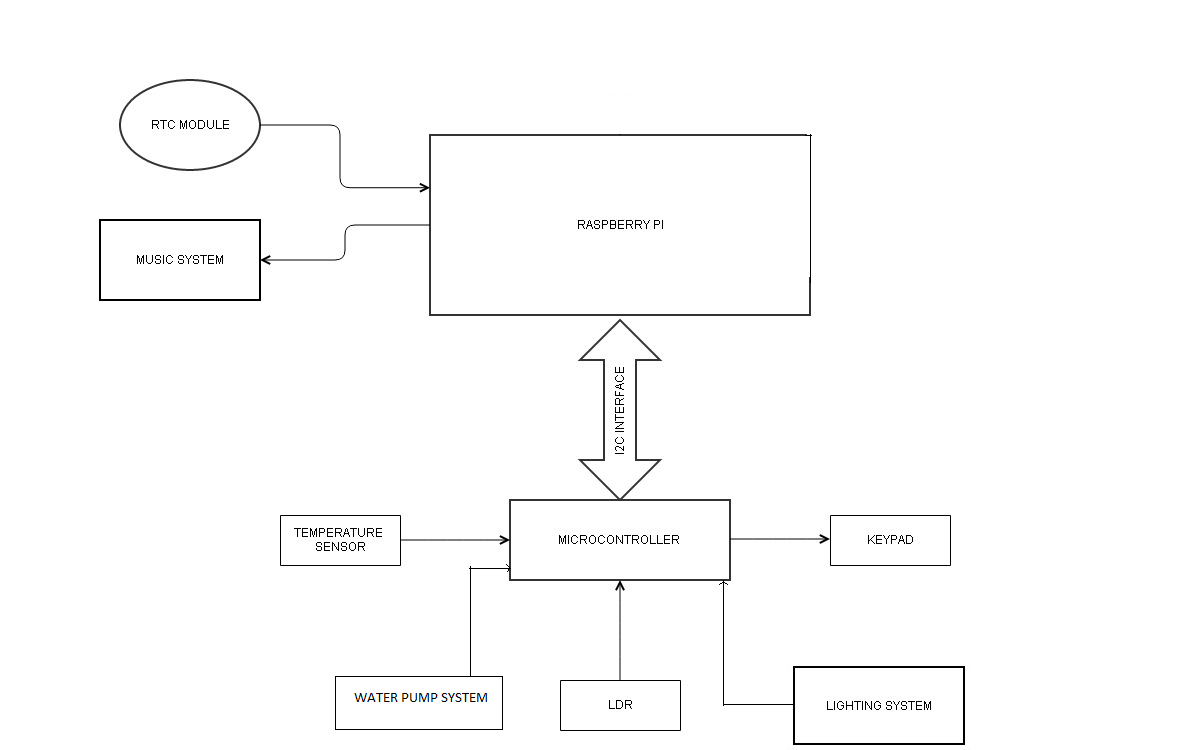
\includegraphics[width=15cm, height=6cm]{fig1.png}
\centering
\label{fig1}
\end{figure}

AT BUS STOP:



\begin{figure}[h]
\begin{center}
\leavevmode
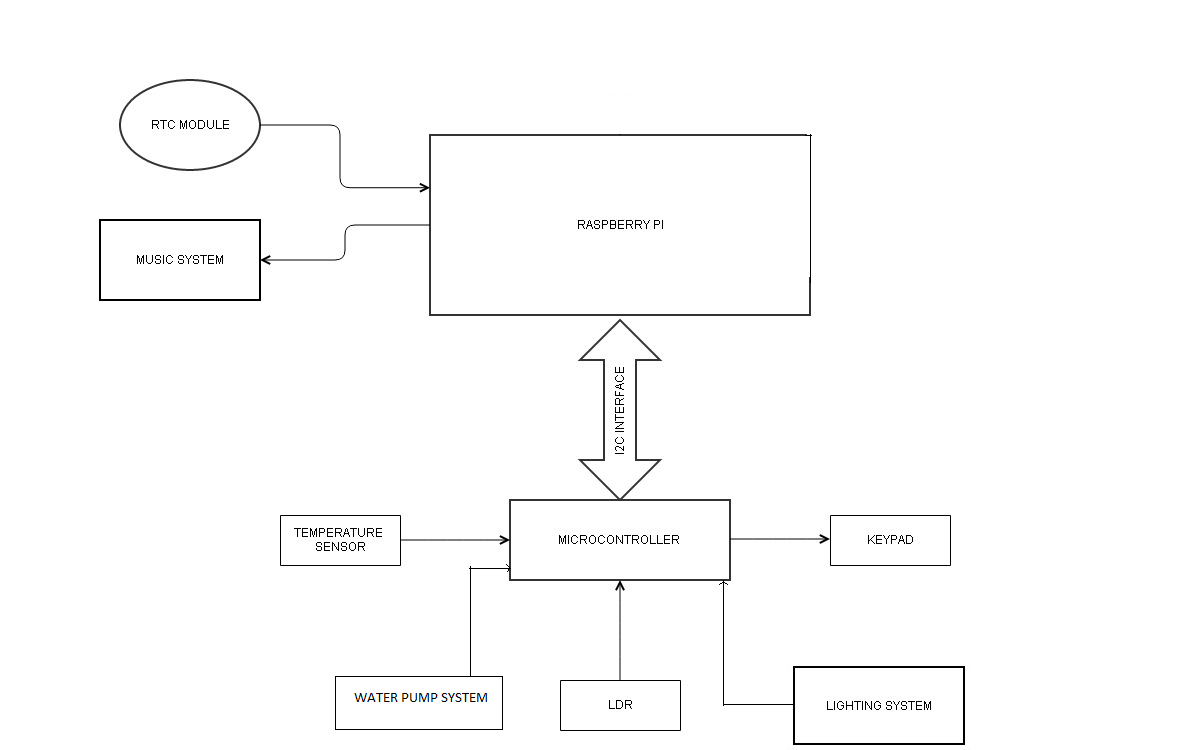
\includegraphics[width=10cm, height=6cm]{fig2.png}
\end{center}
\label{fig2}
\end{figure}

\begin{figure}[h]
\begin{center}
\leavevmode
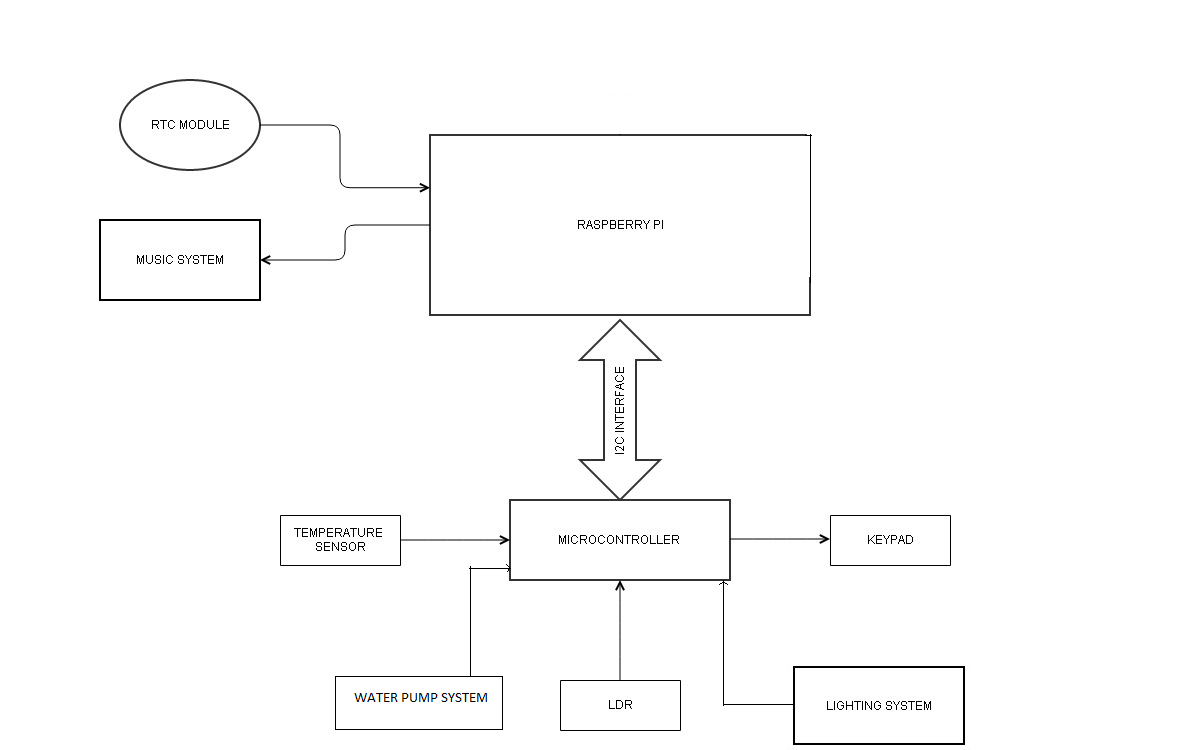
\includegraphics[width=15cm, height=6cm]{fig3.png}
\end{center}

\label{fig3}
\end{figure}

\newpage
\section{WORKING}
\par
\hspace{.7cm}
In this project we present a system which displays the location and other details of the buses which are plying along a particular route. This system is based on micro-controllers and GSM Communication. We intend to use two GSM modules, one in the bus and one at the bus-stop. The hardware inside the bus consisting of a microcontroller and a GSM module will be preloaded with the stop information along the route that the bus will be plying. And the bus stop will also consist of a microcontroller and GSM module that will receive the data and display the relevant information on a suitable display device or in any manner suitable to be communicated with a passenger waiting at the bus stop.
   A transmitter is placed in the bus stop and a receiver in the bus. The transmitter pairs with the receiver, as the bus reaches a stop. This acts as a handshake required for sending the messages. Once this handshake is established, gsm modem sends messages from the onboard module via the microcontroller placed in the bus which then transmits the information to the gsm module placed at the bus stop. This information is passed to a microcontroller for display through the lcd display kit. 

\section{MAIN COMPONENTS REQUIRED}
{$\;\;\;\;$}	
\begin{table}[h]
\begin{tabular}{|c|c|c|}
\hline
\textbf{COMPONENT} & \textbf{QUANTITY} & \textbf{PRICE(Rs.)}\\
\hline
GSM MODEM & 2 & 2400\\
MICROCONTROLLER( PIC 16F877A) & 2 & 480\\
TX-RX MODULE (433 MHz) & 2 & 400\\
LCD DISPLAY & 1 & 330\\
MISCELLANEOUS	& - & 500\\
\hline
\textbf{TOTAL}	& & 4110\\
\hline

\end{tabular}
\end{table}

\textbf{GSM MODEM:}\\
ABCDEFG
devised to work with a GSM wireless network. The GSM wireless modem works in the way like a dial-up modem. The main difference between the GSM modem and dial up modem is that a dial-up modem sends and receives data through a fixed telephone line while a GSM wireless modem sends and receives data through radio wave propagation.  It works similar to a GSM mobile phone, and also GSM modem requires a SIM card for operation. It can be used for internet purpose also depending upon our need.\\

\textbf{MICROCONTROLLER:}\\
 It controls the entire activity of the system. The program for the entire system will be stored in the microcontroller. Also it performs the input and output communications. \\
 
\textbf{TX-RX  MODULE:}\\
It uses radio frequency for transmission and reception. It is the most commonly used form of wireless communication. It doesn't require line of sight propagation. The RF module is often used with a pair of encoder/decoder. The encoder is used for encoding parallel data for transmission feed while reception is decoded by a decoder.  \\



\section{APPLICATIONS}
\par
\hspace{.7cm}
\begin{enumerate}	
\item[1]. This provides prompt, faster and economically feasible transportation for the citizens. This will encourage people to switch over to public transportation system which in turn will lessen the traffic thereby reducing accidents.
\item[2]. Public transportation systems generate income for the government. Increase in the use of public transportation leads to greater income for the government which can be used to provide better services.
\item[3]. Better control over public transportation - Since the public sector transportation is owned and operated by the government this gives them a greater control over public transportation.
\item[4]. Reduces resource consumption
\item[5]. Reduces pollution - Decrease in traffic helps in reducing pollution.
\end{enumerate}

\section{DRAWBACKS}
\par
\hspace{.7cm}
 The proposed system uses more components which makes it more complex hardware -wise i.e. failure of any one of the components can lead to improper message transfer. This in turn demands frequent monitoring and maintenance work.
The system works only when the transmitter and receiver are present within a given range which is not very appreciable.

\newpage
\section{FUTURE PROSPECTS}
\par
\hspace{.7cm}
   If this application is being used in city buses plying in our cities along with a centralized monitoring system and control, this will enable the authorities or a third party to track the vehicle's location, collecting data in the process from the field and delivering it to the base operator to track the fleet throughout the city in real-time on the city map and it will also help the commuter as a navigation aid tool and bus stop information in audio and visual mode. 
  Including gps module can help in real time tracking of the bus. Parameters like velocity, location, number of passengers, bus timings etc. will be readily available to the commuter  thus making this system more  practical and efficient.






\end{onehalfspacing}
\end{document}
